\section{Introducing ggplot2}

Pretty much any statistical plot can be thought of as a mapping between data and one or more visual representations. For example, in a bivariate scatter plot we map two ordered sets of numbers (the variables of interest) to points in thecartesian plane (x,y-coordinates).  In our example above, we further embellished our plot with another mapping in which we mapped the Species labels to different colors.

This notion of representing plots in terms of their mappings is a powerful idea which is central to an approach for plotting that is represented in the R package |ggplot2|.

\subsection{Installing ggplot2}

Like all R packages, |ggplot2| can be installed either from the command line or via the GUI. Here's a reminder of how to do so from the command line:
%
\begin{R}
> install.packages("ggplot2", dependencies=T)
\end{R}

\subsection{Aesthetic and Geometric mappings in ggplot2}

ggplot2 considers two types of mappings from data to visual reprsentations: 1) `aesthetic mappings', which determine the way that data are represented in a plot (e.g. symbols, colors) and 2) `geometry' or `geom' mappings which determine the type of geometric representation that a plot uses.  

The primary plotting function in |ggplot2| is |ggplot()|. The first argument to |ggplot()| is
always a data frame. The data frame is the one that ggplot will use to look for all the mappings that you define in the subsequent pieces of the plot. The nice thing about this is that there is no need to use
the dollar sign notation. As you've seen, you can get similar behavior in base plots by specifying the `data' argument.

The second argument to |ggplot()| is always a function called |aes()|. |aes()| takes named
arguments. Each argument name is the `aesthetic' that you want mapped to a particular variable (column) in the data. 

The final piece of information that we need to draw our plot is the `geom'. All geoms are encoded as R functions. The syntax used to add them to a plot is simply a `+' sign.  There are many different ggplot geoms for different plot types. We'll explore a few of the built-in geoms in this chapter; additional geoms will come up in later weeks.


\subsection{Scatter plots using ggplot2}

Let's recreate our iris scatter plot using the function |ggplot| from the ggplot2 library:
\begin{R}
> library(ggplot2)
> ggplot(iris, aes(x = Sepal.Length, y = Petal.Length, 
                col = Species)) + geom_point()
\end{R}
%
Following the requirement outline above, |iris| is our data frame, the call to |aes| set's up our aesthetic mapping, and we're specifying the use of the point geom (|geom_point()|) to map the x- and y-values in the aesthetic mapping to points in the cartesian plane. In the function call above, we told ggplot that we wanted the sepal length on the x axis, the petal length on the y axis, and the colors to be encoded by the species. However, we could choose any number of other aesthetic mappings. For example, could use shape instead of color to represent the Species labels:
\begin{R}
> ggplot(iris, aes(x = Sepal.Length, y = Petal.Length, 
                shape = Species)) + geom_point()
\end{R}
%
or alternately, size:
%
\begin{R}
> ggplot(iris, aes(x = Sepal.Length, y = Petal.Length, 
                size = Species)) + geom_point()
\end{R}
%
We can even combine multiple aesthetics in a single plot:
%
\begin{R}
> ggplot(iris, aes(x = Sepal.Length, y = Petal.Length, 
                col = Species, shape = Species)) + geom_point()
\end{R}
The resulting plot is shown in Figure~\ref{fig:ggplotscatter}.
%
\begin{figure}[htbp]
\centering
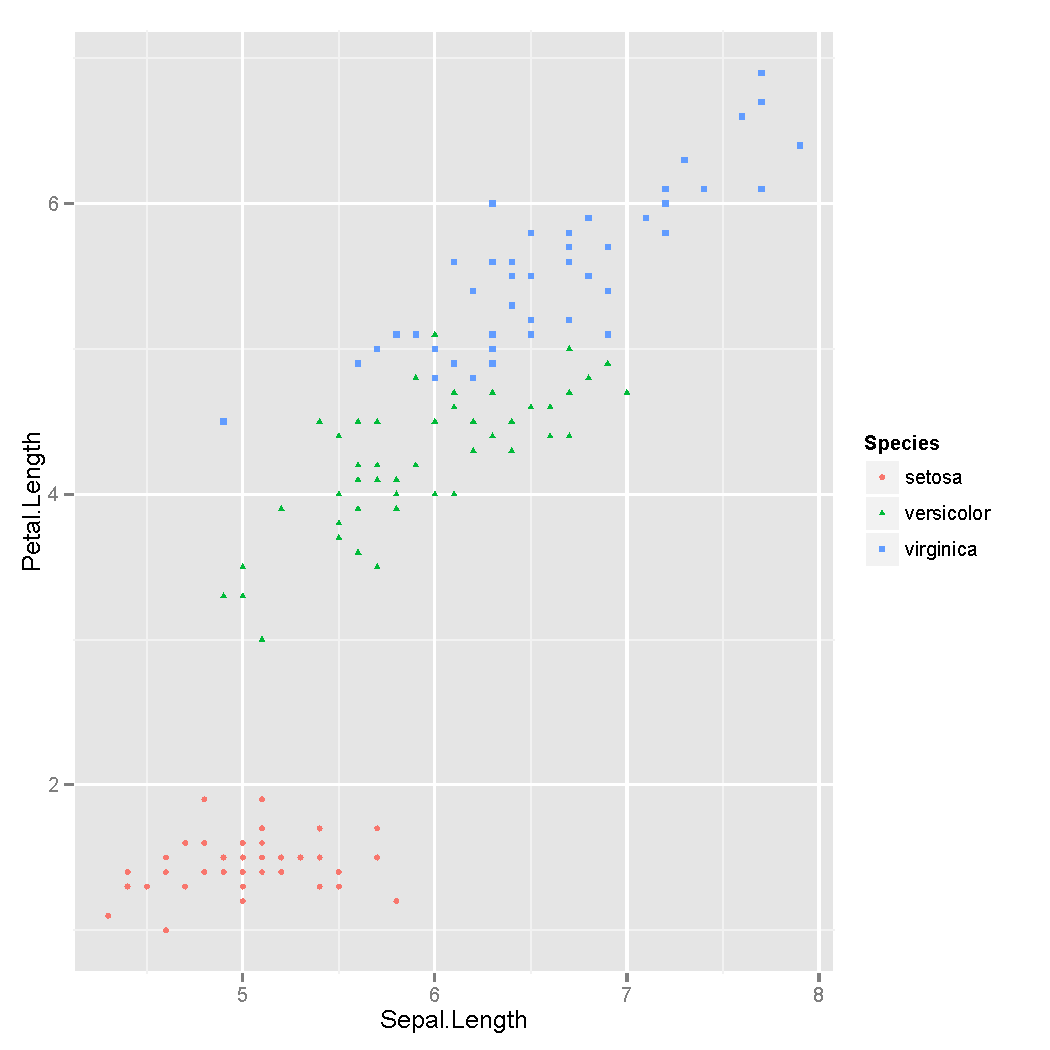
\includegraphics[width=0.5\columnwidth]{./figures/hands-on2/ggplot-scatter.pdf}
\caption{Scatter plot created from the iris data set using the \lstinline!ggplot! function.}
\label{fig:ggplotscatter}
\end{figure}


There's a number of advantages to using |ggplot|  rather than trying
to replicate this plot with base graphics functions in R:
%
\begin{enumerate}
\item The legend is automatically drawn for you.
\item The code is very easy to change. Rather than having to figure out
   how to manually map a point size onto a variable using some
   difficult R code, it's just as simple as saying to set the `size'
   equal to a `variable'.
\item It's easy to swap around variables from one aesthetic mapping to another.
\end{enumerate}
%

Having a good understanding of both the base plotting functions and a powerful package like |ggplot2| allows you maximum flexibility in terms of the statistical graphics you are able to produce.


\subsection{Some additional ggplot geoms}

So far we've only looked at a single geom (|geom_point()|).  Let's revisiting some of the univariate plots from last week using ggplot.

\paragraph{Boxplots}

|geom_boxplot()| constructs boxplots in ggplot.
%
\begin{R}
> ggplot(iris, aes(x = Species, y = Sepal.Length, col=Species)) + 
      geom_boxplot()
\end{R}


\paragraph{Histograms}

|geom_histogram()| is used to construct histogram plots in ggplot.
%
\begin{R}
> ggplot(iris, aes(x = Sepal.Length)) + geom_histogram()
\end{R}
%
Here we let |ggplot| pick the default bin widths.  Below we show how to change the bin width:
%
\begin{R}
> ggplot(iris, aes(x = Sepal.Length)) + geom_histogram(binwidth=0.25)
\end{R}
If we want to color histogram by species identity you need to set the |position = 'identity'| in the call to |geom_histogram|:
\begin{R}
> ggplot(iris, aes(x = Sepal.Length, fill=Species)) + 
        geom_histogram(binwidth=0.25, position='identity',alpha=0.65)
\end{R}
The above code also set the transparency of the bar fills using the |alpha| argument.  As an alternative to overlaying the histogram bins for each species, you can show the bins side-by-side using the argument |position = 'dodge'|.
\begin{R}
> ggplot(iris, aes(x = Sepal.Length, fill=Species)) + 
        geom_histogram(binwidth=0.25, position='dodge')
\end{R}

\paragraph{Density plots}

|geom_density()| creates density plots in ggplot.
%
\begin{R}
> ggplot(iris, aes(x = Sepal.Length, fill=Species)) + 
        geom_density(alpha=0.65)
\end{R}

There's also a 2D version of the density plot, created using |geom_density2d()|.  This can be usefully combined with |geom_points()| to create a bivariate scatter plot with density contours.
%
\begin{R}
> ggplot(iris, aes(x = Sepal.Length, y = Petal.Length, col = Species)) + 
    geom_point() + geom_density2d(alpha=0.25)
\end{R}

\paragraph{Scatter plots with marginal density plots}

The file |scatterWithMargins.R| from the course wiki contains a function that uses multiple calls to |ggplot()| to combine two marginal density plots with a scatter plot.  To use this function you'll need to install a package called "gridExtra":
%
\begin{R}
> install.packages("gridExtra", dependencies=T)
\end{R}
Then import the new function from |scatterWithMargins.R| and use it as so:
%
\begin{R}
> scatterWithMargins(iris, "Sepal.Length", "Petal.Length", "Species")
\end{R}
This produces the plot shown in Figure~\ref{fig:ggplotfancy}.
%
\begin{figure}[htbp]
\centering
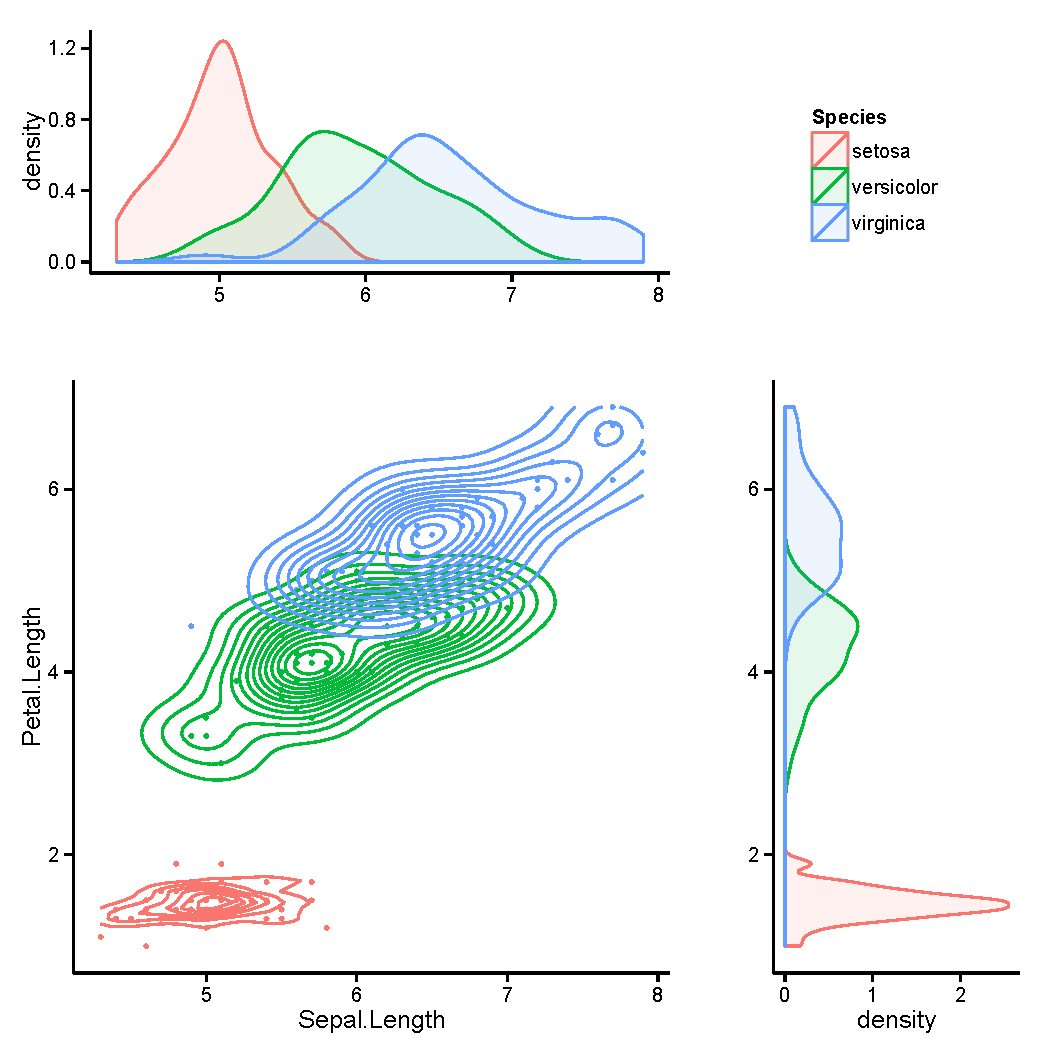
\includegraphics[width=0.5\columnwidth]{./figures/hands-on2/ggplot-fancy.pdf}
\caption{Figure produced by the \lstinline!scatterWithMargins! function from the course wiki.}
\label{fig:ggplotfancy}
\end{figure}

\newpage